\input{commun/presentations.tex}

\title[Séance 8 - Carto \& Nav]{Séance 8 \\ Cartographie \& Navigation}

\begin{document}
 \begin{frame}
 \titlepage
 \end{frame}
 
 \begin{frame}{La cartographie et la navigation}
 	\question{Que faut-il pour naviguer en avion ?}
 	
 	\pause
 	\question{De quelles informations avons nous besoin ?}
 	\question{Quels outils peut-on utiliser ?}
 
 \end{frame}
 
 \begin{frame}
 \tableofcontents
 \end{frame}
 
 \section{Cartographie}
 	\begin{frame}{Latitude et longitude : se situer sur la planète}
	
		\begin{figure}[H]
			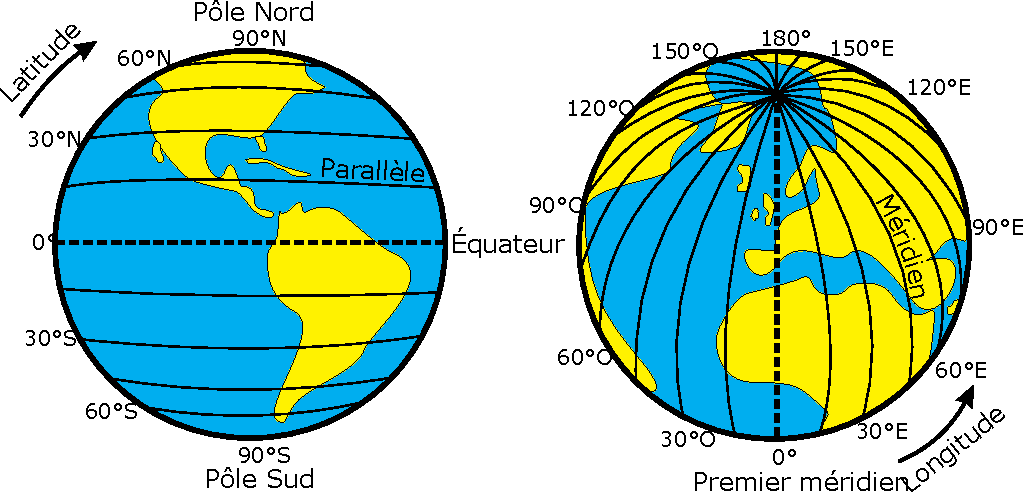
\includegraphics[width=0.95\linewidth]{02-Navigation/img/latitudeAndLongitudeOfTheEarth.pdf}
			\legende{Latitudes et longitudes sur la Terre}{img:latitudeAndLongitudeOfTheEarth}
		\end{figure}	
	\end{frame}
 	
	\begin{frame}{Le mille nautique}
	\begin{columns}
		\begin{column}{0.4\textwidth}
		\begin{figure}[H]
			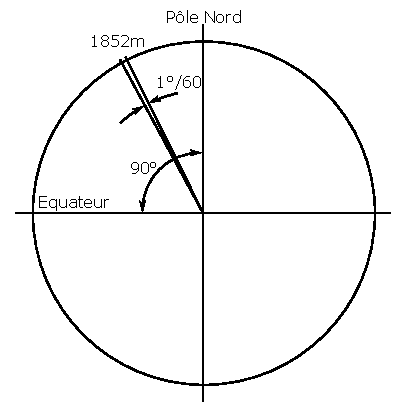
\includegraphics[width=0.95\linewidth]{02-Navigation/img/definitionMilleNautique.pdf}
			\legende{Le mille nautique}{img:definitionMilleNautique}
		\end{figure}	
		\end{column}
		\begin{column}{0.6\textwidth}
			\begin{itemize}
				\item Chaque degré de latitude ou longitude est divisé en 60 : les minutes d'arc. On peut encore subdiviser chaque minute d'arc en 60 secondes
				\item Les navigateurs ont défini la longueur définie par une minutes d'arc sur un méridien comme étant un \textbf{mille nautique}
				\item 1 mille nautique (ou marin) vaut 1~852 mètres
				\item le mille nautique est nommé NM
				\item unité de vitesse : le n\oe d. Un n\oe d correspond à 1 NM/h
			\end{itemize}
		\end{column}
	\end{columns}
	\end{frame}
	
	\begin{frame}{Carte de navigation au 1/500~000}
	\begin{columns}
		\begin{column}{0.6\textwidth}
		\begin{figure}[H]
			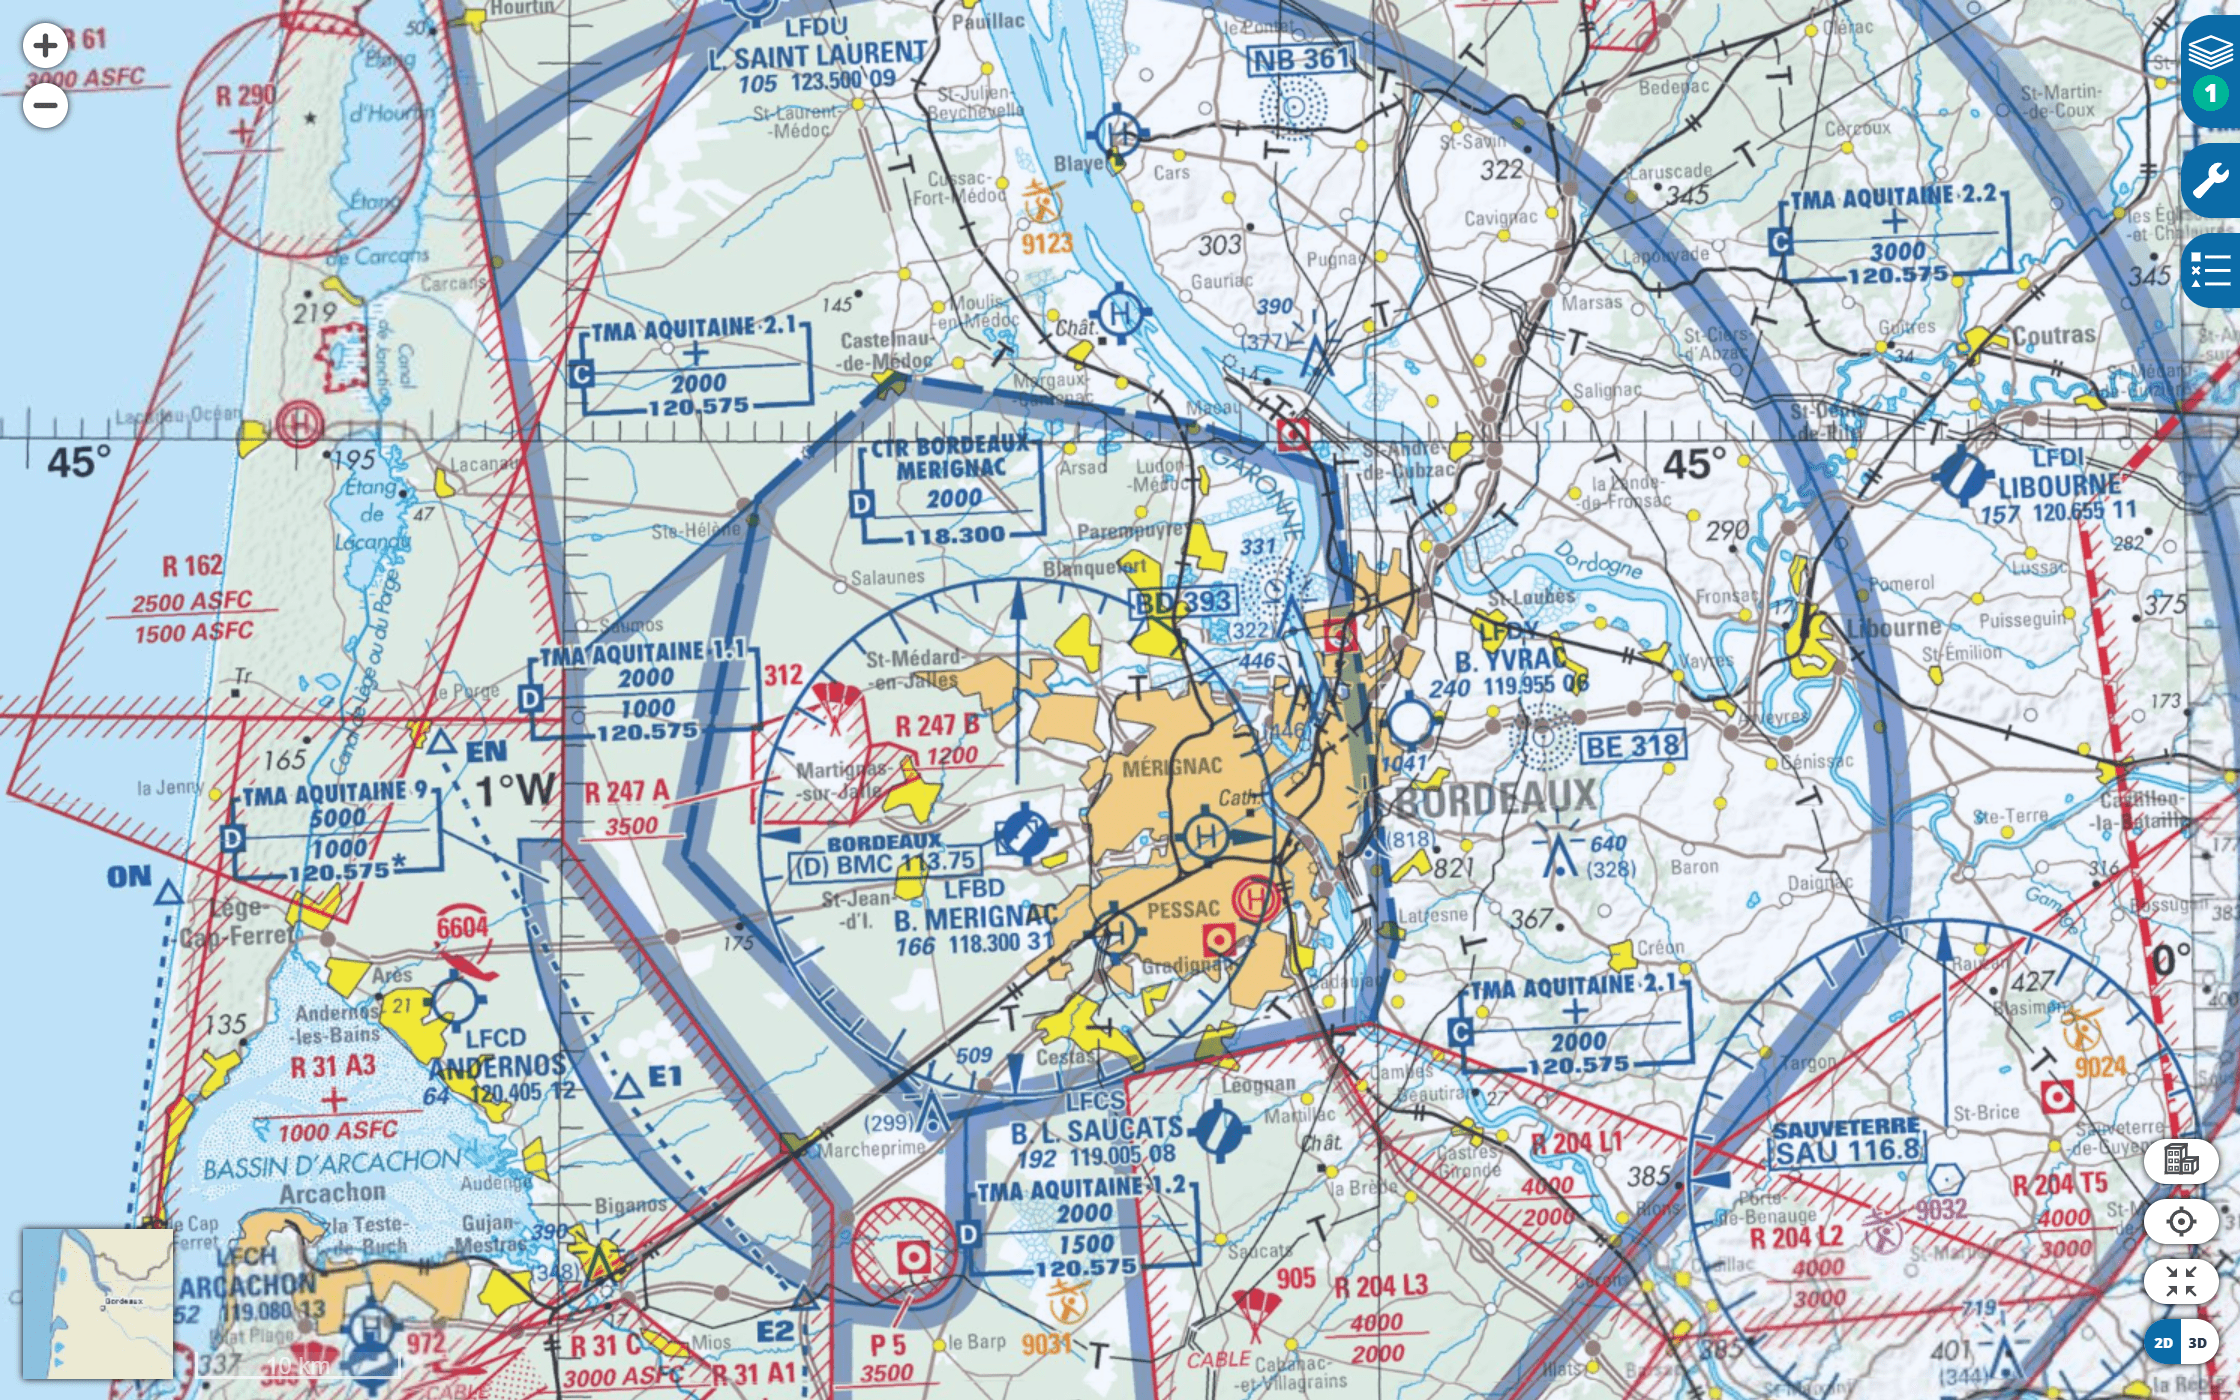
\includegraphics[width=0.95\linewidth]{Annexes/img/ignOaciBordeaux.png}
			\legende{Extrait de carte OACI VFR}{img:ignOaciBordeaux}
		\end{figure}	
		\end{column}
		\begin{column}{0.4\textwidth}
			\begin{itemize}
				\item Carte de navigation à vue
				\item Échelle 1/500~000 \pause $1~cm = 500~000~cm \pause \Leftrightarrow  1~cm = 5~km$
			\end{itemize}
		\end{column}
	\end{columns}
	\end{frame}
 
	
\appendix 
\section{QCM}
\qmcBia{Navigation, réglementation, sécurité des vols}
{4}{Quelle est la correspondance d'un mille nautique dans le système métrique ?}
{$1~528~m$}
{$1~609~m$}
{$0,8~m^2$}
{$1,852~km$} 
{}

\qmcBia{Navigation, réglementation, sécurité des vols}
{3}{Sur une carte au 1/500~000ème une distance mesurée de 15 cm correspond à une distance réelle de :}
{15 km}
{30 km}
{75 km}
{150 km} 
{Sur une carte au 1/500~000, $1~cm = 500~000~cm \Leftrightarrow 1~cm = 5~km$. Donc $15~cm \times 5~km = 75~km$}

\qmcBia{Navigation, réglementation, sécurité des vols}
{2}{Sur la carte VAC, vous pouvez identifier les coordonnées en latitude et longitude de l'aéroport, la latitude de 43\textdegree 39’ et 55’’ N est relevée par rapport :}
{au méridien de Greenwich}
{à l'équateur}
{au pôle Nord}
{au tropique du Cancer} 
{}

\qmcBia{Navigation, réglementation, sécurité des vols}
{3}{Comment est appelé l'angle entre le nord vrai et le nord magnétique ? }
{déclinaison magnétique}
{déviation}
{erreur de parallaxe}
{inclinaison magnétique} 
{}

\qmcBia{Navigation, réglementation, sécurité des vols}
{1}{En vol, le vent vous oblige à suivre un cap magnétique inférieur à la route magnétique prévue afin de la suivre. Vous en déduisez que le vent : }
{vient de votre gauche}
{vient de votre droite}
{est de face} 
{est arrière}
{Si la route est au 090\textdegree et qu'on prend un cap au 080\textdegree pour contrer, c'est qu'on a le nez tourné vers la gauche pour "lutter" contre un vent venant de la gauche}

\qmcBia{Navigation, réglementation, sécurité des vols}
{2}{Vous effectuez un vol à l'estime. Cela consiste à : }
{suivre des lignes naturelles ou des repères caractéristiques du sol}
{déterminer le cap à prendre et l'heure estimée d'arrivée à un point caractéristique en fonction de sa vitesse}
{estimer sa position à l'aide d’un VOR (VHF Omnidirectional Range)} 
{estimer sa position à l'aide d'un goniomètre}
{1) est le cheminement, 3) la radionavigation}
 
\input{commun/beamerSlidesBiblio.tex} 
 
\end{document}
